\section{Experimental Evaluation}

%%%%%%%%%%%%%%%
\begin{frame}{}
  \begin{center}
    Impacts of \rvsi{} specification \\[5pt]
    on the \emph{\blue{transaction abort rates}} in various scenarios
  \end{center}

  \pause
  \vspace{0.50cm}
  \centerline{\red{What about performance?}}
  \begin{itemize}
    \item Not reported in this work
    \item \emph{Not} sensitive to parameters
  \end{itemize}
\end{frame}
%%%%%%%%%%%%%%%

%%%%%%%%%%%%%%%
\begin{frame}{}
  \begin{columns}
    \column{0.50\textwidth}
      \chameleon{} prototype on Aliyun:
      \begin{itemize}
	\item 3 datacenters~\footnotemark[1]
	\item 3 nodes in each datacenter
	\item Partition \& Replication
	\item Clients in our lab~\footnotemark[2]
      \end{itemize}
    \column{0.50\textwidth}
      \fignocaption{width = 0.85\textwidth}{figs/chameleon-arch.pdf}
  \end{columns}

  \footnotetext[1]{Located in East China, North China, and South China, respectively.}
  \footnotetext[2]{Located in East China.}
\end{frame}
%%%%%%%%%%%%%%%

%%%%%%%%%%%%%%%
\begin{frame}{}
  \centerline{Three categories of workload parameters for experiments on Aliyun.}
  \begin{table}[!t]
  \centering
  \renewcommand*{\arraystretch}{1.2}
  \caption{Three categories of workload parameters for experiments on Aliyun.}
  % \resizebox{0.95\textwidth}{!}{%
    { %
  \begin{tabular}{|c|c||c|c|}
	\hline
    \multicolumn{2}{|c||}{\textbf{Parameter}} & \textbf{Value}		& \textbf{Explanation}
	\\ \hline  \hline
    \multirow{6}{*}{\bf Transaction-related}
    &\#keys  						& 25 = 5 (rows) $\times$ 5 (columns)  	&  	size of keyspace
	\\ \cline{2-4}
	&\#clients						& 5, 10, 15, 20, 25, 30 & number of clients
    \\ \cline{2-4}
	&\#txs/client					& 1000 & number of transactions per client
	\\ \cline{2-4}
	&\#ops/tx				& $\sim$ Binomial(20, 0.5) &  number of operations per transaction
	\\ \cline{2-4}
	&rwRatio							& 1:2, 1:1, 4:1 & {\#reads}/{\#writes}
	\\ \cline{2-4}
	&zipfExponent					& 1		& parameter for Zipfian distribution
	\\ \hline  \hline
    \multirow{3}{*}{\bf Execution-related} & minInterval						& 0ms		& minimum inter-transaction time
	\\ \cline{2-4}
	&maxInterval						& 10ms		& maximum inter-transaction time
	\\ \cline{2-4}
	&meanInterval					& 5ms		& mean inter-transaction time
    \\ \hline \hline
    {\bf RVSI-related} & $(k_1, k_2, k_3)$		
		&  \innercell{c}{(1,0,0) (1,1,0) (1,1,1) \\ (2,0,0) (2,0,1) (2,1,1)}	
		&  for $\konebv{}$, $\ktwofv{}$, and $\kthreesv{}$
	\\ \hline
  \end{tabular}}
  % }
\end{table}

\end{frame}
%%%%%%%%%%%%%%%

%%%%%%%%%%%%%%%
\begin{frame}{}
  Roadmap:
  \begin{enumerate}[<+->]
    \setlength{\itemsep}{5pt}
    \item Transaction abort rates because of \blue{violating the \rvsi{} version constraints}
      are quite \red{\it sensitive} to different values of $k_1$, $k_2$, or $k_3$.
    \item In the \blue{Aliyun scenarios}, most transactions have been aborted because of violating \red{$\ktwofv$}.
    \item In \blue{controlled experiments}, the impacts of \red{$\konebv$} emerge when the ``issueDelay'' gets shorter.
  \end{enumerate}

  \vspace{0.50cm}
  \uncover<4->{
    \centerline{We report the results under the read-frequent 
      (\#rwRatio = 4:1) workloads~\footnote{\url{https://github.com/hengxin/chameleon-transactional-kvstore}}.}
  }
\end{frame}
%%%%%%%%%%%%%%%

%%%%%%%%%%%%%%%
\begin{frame}{}
  \fignocaption{width = 0.80\textwidth}{figs/aliyun-vc-rf.pdf}

  \pause
  The transaction abort rates due to ``vc-aborted'' \pause can be \red{greatly reduced}
  by \blue{slightly} increasing the values of $k_1$, $k_2$, or $k_3$:
  \[
    vc(1,0,0) = 0.1994 \implies vc(2,1,1) = 0.0091 \quad (\text{\#clients} = 30)
  \]
\end{frame}
%%%%%%%%%%%%%%%

%%%%%%%%%%%%%%%
\begin{frame}{}
  \fignocaption{width = 0.55\textwidth}{figs/aliyun-bvfvsv.pdf}

  \pause
  \centerline{Most ``vc-aborted'' transactions abort because of violating \red{$\ktwofv$}.}
  \[
    fv(1,0,0) = 0.1889 \implies fv(\blue{2},0,0) = 0.1866 \implies fv(1,\red{\bf 1},0) = 0.0064
  \]
\end{frame}
%%%%%%%%%%%%%%%

%%%%%%%%%%%%%%%
\begin{frame}{}
  \begin{center}
    In the Aliyun scenarios, we saw \red{\it little} impacts of $\konebv$. \\[30pt]

    \pause
    We therefore explore the impacts of $\konebv$ in controlled experiments.
  \end{center}
\end{frame}
%%%%%%%%%%%%%%%

%%%%%%%%%%%%%%%
\begin{frame}{}
  \centerline{Three types of delays for \blue{\large controlled experiments} on local hosts.}
  \begin{center}
    \begin{tikzpicture}[
  delay/.style = {>=Stealth, ->, very thick}]
  \node (client) [] {
\includegraphics[scale = 0.15]{figs/client-pc-logo.png}};
  \node (lms) [below left = 1.8cm and -0.5cm of client] {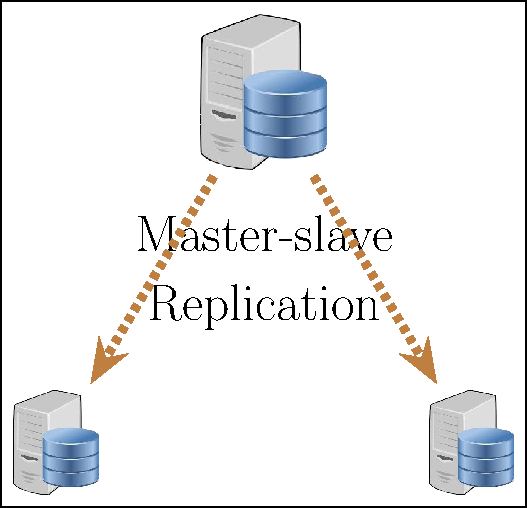
\includegraphics[scale = 0.30]{figs/master-slave.pdf}};
  \node (rms) [below right = 1.8cm and -0.5cm of client] {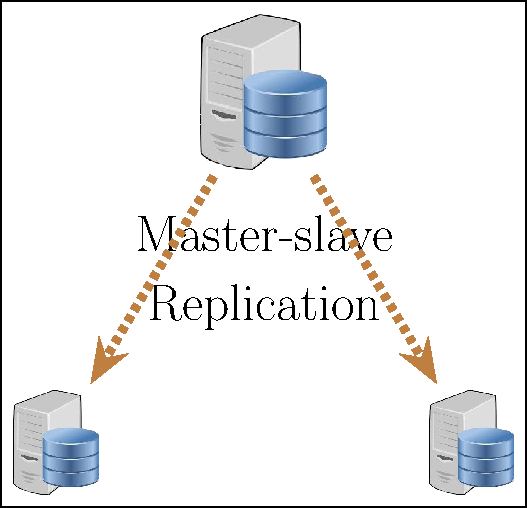
\includegraphics[scale = 0.30]{figs/master-slave.pdf}};

  \uncover<2->{
    % issue delay
    \draw [delay, cyan] (client) to node () [right = -8pt] {issueDelay} ($(lms.north) - (0, 2pt)$);
    \draw [delay, cyan] (client) to ($(rms.south west) + (10pt, 25pt)$);
  }

  \uncover<3->{
    % replication delay
    \draw [delay, teal] ($(rms.north) - (-15pt, 20pt)$) to [bend left] 
    node () [above, sloped] {replDelay} ($(rms.south east) - (15pt, -25pt)$);
  }

  \uncover<4->{
    % 2pc delay
    \draw [delay, blue] ($(lms.north) - (-15pt, 20pt)$) to node () [above] {2pcDelay} ($(rms.north) - (15pt, 20pt)$);
  }
\end{tikzpicture}
  \end{center}

  \begin{table}[!t]
  \centering
  \renewcommand*{\arraystretch}{1.2}
  \begin{tabular}{|c||c|c|}
	\hline
	{\bf Types}		& {\bf Values (ms)}	& {\bf Explanation}
	\\ \hline \hline
	{\bf issueDelay}	& 5, 8, 10, 12, 15, 20	& delays between clients and replicas
	\\ \hline
	{\bf replDelay}	& 5, 10, 15, 20, 30 	& delays between masters and slaves
	\\ \hline
	{\bf 2pcDelay}	& 10, 20, 30, 40, 50 	& delays among masters
	\\ \hline
  \end{tabular}
\end{table}

\end{frame}
%%%%%%%%%%%%%%%

%%%%%%%%%%%%%%%
\begin{frame}{}
  \begin{columns}
    \column{0.50\textwidth}
      \fignocaption{width = 0.90\textwidth}{figs/simlog-rw4.pdf}
      \vspace{-0.40cm}
      \centerline{\footnotesize (Under read-frequent workloads.)}
    \column{0.50\textwidth}
      \fignocaption{width = 0.90\textwidth}{figs/simlog-rw05.pdf}
      \vspace{-0.40cm}
      \centerline{\footnotesize (Under write-frequent workloads.)}
  \end{columns}

  \vspace{0.40cm}
  \begin{center}
    When the \textcolor{teal}{``issueDelay''} gets shorter, \\
    % the impacts of \blue{$\ktwofv$} go weaker, \\
    the impacts of \red{$\konebv$} have begun to emerge.
  \end{center}
\end{frame}
%%%%%%%%%%%%%%%

% %%%%%%%%%%%%%%%
% \begin{frame}{}
%   \begin{description}[issueDelay = 20ms:]
%     \setlength{\itemsep}{10pt}
%     \item[issueDelay = 20ms:] $bv(1,0,0) = \red{0.0057} \quad\;\; fv(1,0,0) = 0.0251$
%     \item[issueDelay = 15ms:] $bv(1,0,0) = \red{0.08225} \quad fv(1,0,0) = 0.0393$
%     \item[issueDelay = 5ms:] $bv(1,0,0) = \red{0.1716} \quad\;\; fv(1,0,0) = 0.0045$
%   \end{description}
% 
%   \pause
%   \vspace{0.50cm}
%   \begin{center}
%     \blue{larger issueDelay} $\implies$ longer transaction \\[5pt]
%     more concurrent transactions \\[5pt]
%     more likely to obtain data versions updated by concurrent transactions \\[5pt]
%     more sensitive to \blue{$\ktwofv$}
%   \end{center}
% \end{frame}
% %%%%%%%%%%%%%%%

%%%%%%%%%%%%%%%
\begin{frame}{}
  Generally, \rvsi{} \blue{\it helps to reduce the transaction abort rates}
  when applications are willing to tolerate certain anomalies.

  \pause
  \vspace{0.6cm}
  \begin{description}[<+->]
    \setlength{\itemsep}{5pt}
    \item[$\ktwofv$:] In the Aliyun scenarios, most transactions have been aborted because of violating $\ktwofv$.
    \item[$\konebv$:] In controlled experiments, the impacts of $\konebv$ emerge when the ``issueDelay'' gets shorter.
    \item[$\kthreesv$:] \uncover<4->{\textcolor{gray}{Complex and challenging (involving multiple data items)}}
  \end{description}
\end{frame}
%%%%%%%%%%%%%%%
